\section{Experimental results} \label{experiments}

\subsection{Dataset insights}  \label{ch:experimentsA}

This chapter presents the dataset insights of the complete dataset with full genome sequences and the dataset insights of the preprocessed dataset.

\subsubsection{Complete dataset}  \label{ch:experimentsAa}

\begin{wrapfigure}{R}{8cm}
	\centering
	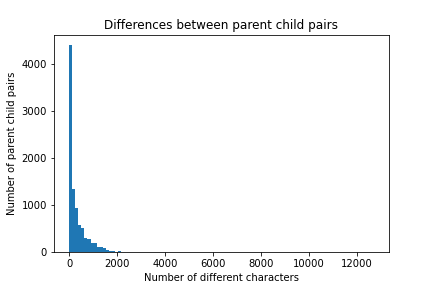
\includegraphics[width=0.9\linewidth]{figures/distributionDifferencesParentChild.png}
	\caption{Distribution of the differences between parent and child sequences \cite{own representation}}
	\label{distributionDifferencesParentChild}
\end{wrapfigure}

The dataset consists of 9199 parent child pairs.
The distribution how the parent and child sequences differ can be seen in figure \ref{distributionDifferencesParentChild}. The majority of parent child pairs differ in less than 200 characters. The number of completely equal parent child pairs is 396.

\vspace{2cm}
Figure \ref{mutatedGeneticLoci} visualizes the distribution of mutations over the full \ac{SARS-CoV-2} genome.

\begin{figure}[ht!]
	\centering
	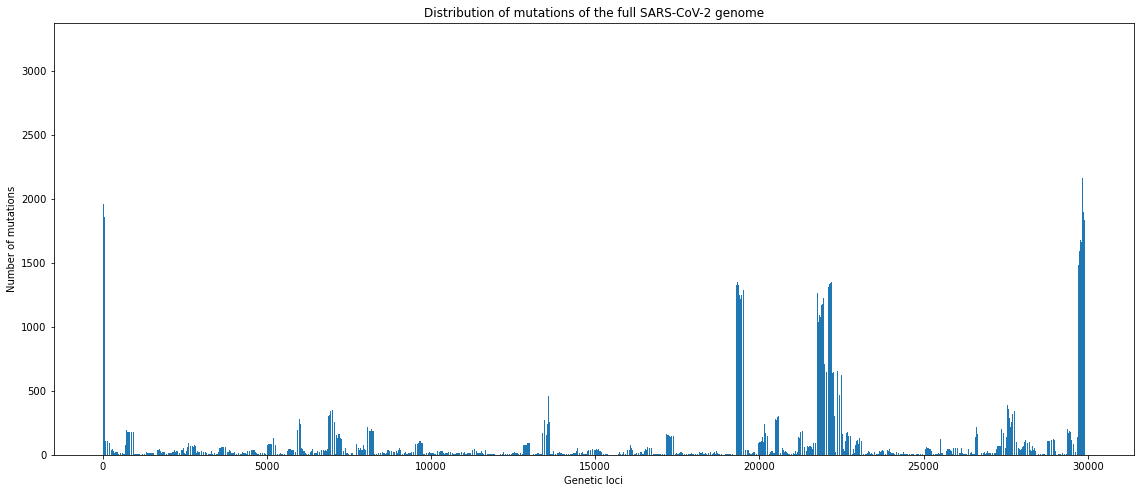
\includegraphics[width=1.0\linewidth]{figures/mutatedGeneticLoci.png}
	\caption{Mutated genetic loci \cite{own representation}}
	\label{mutatedGeneticLoci}
\end{figure}

\newpage
\subsubsection{Preprocessed dataset}  \label{ch:experimentsAb}

The complete dataset is preprocessed as described in chapter \ref{ch:approachB}. The distribution how the parent and child amino acids differ in the selected subpart can be seen in figure \ref{preprocessedDistributionDifferencesParentChild}. The majority (6946) of parent child pairs are equal.

\begin{figure}[ht]
	\centering
	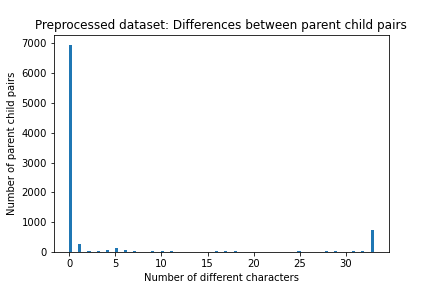
\includegraphics[width=0.6\linewidth]{figures/preprocessedDistributionDifferencesParentChild.png}
	\caption{Preprocessed dataset: Distribution of the differences between parent and child sequences \cite{own representation}}
	\label{preprocessedDistributionDifferencesParentChild}
\end{figure}

Figure \ref{preprocessedMutatedGeneticLoci} visualizes the differing amino acids and their positions of the selected subpart of the \ac{SARS-CoV-2} genome. They are distributed equally over the selected subpart.

\begin{figure}[ht]
	\centering
	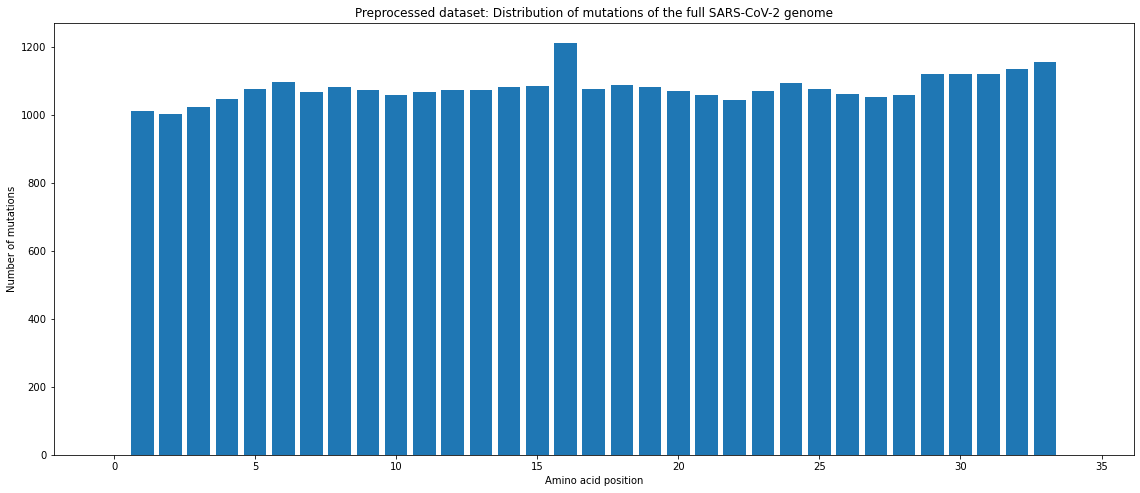
\includegraphics[width=1.0\linewidth]{figures/preprocessedMutatedGeneticLoci.png}
	\caption{Preprocessed dataset: Differing amino acid positions \cite{own representation}}
	\label{preprocessedMutatedGeneticLoci}
\end{figure}

\newpage
\subsection{Evaluation}  \label{ch:experimentsB}

For evaluating the model prediction we need to compare the generated se\-quence with the real sequence. For this text similarity task there are already metrics available in the \ac{NLP} area. Berman et al. \cite{Berman2020} have used the \ac{BLEU} score. This metric comes from the area of machine translation and evaluates the similarity between machine generated text and human generated text. The more similar the two texts are, the better the \ac{BLEU} score is. It is always in the range between zero and one. With one as perfect similarity and zero means no similarity.

\subsubsection{Transformer pretraining}  \label{ch:experimentsBa}

Figure \ref{pretrainingLossPlot} shows the loss plot for the Transformer pretraining. The model converges rather fast. The first meaningful results are already reached after 2 epochs. The reached BLEU score is 0.8559. From this point of view the results look very promising. That is why the details of these results are investigated. When comparing all predictions with the true values it is noticeable, that the model prediction is always the same for all 460 test instances. This could be explained by the fact, that the predicted sequence is correct in 318 of 460 cases. Therefore it can be assumed, that the model works, but the used dataset is not optimal.

\begin{figure}[ht]
	\centering
	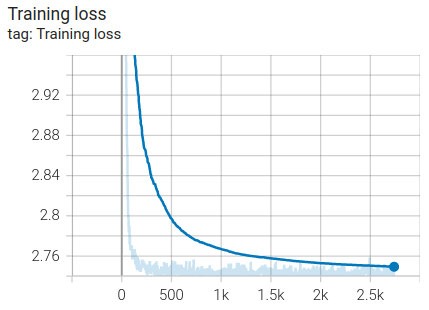
\includegraphics[width=0.5\linewidth]{figures/pretrainingLossPlot.png}
	\caption{Transformer pretraining loss plot}
	\label{pretrainingLossPlot}
\end{figure}


\subsubsection{GAN training}  \label{ch:experimentsBb}

TODO

% Define what is a correct mutation prediction, see MutaGAN paper - Generator Evaluation
% Define Evlauation metrics, see MutaGAN paper - Generator Evaluation
% Evaluation chaper of MutaGAN very well written, will be inspiring
% Compare our performance to those of other papers

\newpage
